\documentclass[12pt,a4paper]{article}

% ===== 中文支持 =====
\usepackage[UTF8,zihao=-4]{ctex}

% ===== 页边距（GB/T 7713.1）=====
\usepackage[
  top=2.5cm,bottom=2.5cm,
  left=2.8cm,right=2.8cm
]{geometry}

% ===== 字体 =====
\usepackage{fontspec}
\setmainfont{Times New Roman}

% ===== 行距与段落 =====
\usepackage{setspace}
\setstretch{1.5}
\setlength{\parskip}{0pt}

% ===== 插图与表格 =====
\usepackage{graphicx}
\usepackage{float}
\usepackage{booktabs}
\usepackage{array}
\usepackage{makecell}
\usepackage{adjustbox}
\graphicspath{{report_yzh_assets/}}

% ===== 数学公式 =====
\usepackage{amsmath,amssymb}

% ===== 图表编号 =====
\usepackage{chngcntr}
\renewcommand{\thefigure}{\arabic{section}-\arabic{figure}}
\renewcommand{\thetable}{\arabic{section}-\arabic{table}}
\counterwithin{figure}{section}
\counterwithin{table}{section}

% ===== 图表标题格式 =====
\usepackage{caption}
\usepackage{subcaption}
\captionsetup{
  font=small,
  labelsep=space,
  justification=centering,
  aboveskip=6pt,
  belowskip=12pt
}
\captionsetup[table]{
  aboveskip=12pt,
  belowskip=6pt,
  position=above
}

% ===== 页眉页脚 =====
\usepackage{fancyhdr}
\setlength{\headheight}{15pt}
\pagestyle{fancy}
\fancyhf{}
\fancyhead[C]{\small 实验报告}
\fancyfoot[C]{\small\thepage}

% ===== 目录超链接 =====
\usepackage[
  colorlinks=true,linkcolor=black,citecolor=black,urlcolor=blue,
  bookmarks=true,bookmarksnumbered=true
]{hyperref}

% ===== 章节标题格式 =====
\usepackage{titlesec}
\titleformat{\section}[block]
  {\centering\heiti\zihao{3}}{\thesection}{1em}{}
\titlespacing*{\section}{0pt}{24pt}{18pt}
\titleformat{\subsection}[hang]
  {\heiti\zihao{4}}{\thesubsection}{1em}{}
\titlespacing*{\subsection}{0pt}{18pt}{6pt}
\titleformat{\subsubsection}[hang]
  {\heiti\zihao{-4}}{\thesubsubsection}{1em}{}
\titlespacing*{\subsubsection}{0pt}{12pt}{6pt}

\begin{document}

\begin{titlepage}
  \centering
  \vspace*{3cm}
  {\heiti\zihao{2} 实验报告}\\[1cm]
  {\heiti\zihao{3} 星点法测量透镜像差综合实验}\\[2cm]
  \begin{tabular}{ll}
    姓\quad 名： & 叶哲昊 \\[0.5cm]
    实验日期： & 2026年6月26日
  \end{tabular}
  \vfill
\end{titlepage}

\pagestyle{empty}
\tableofcontents
\newpage
\pagestyle{fancy}
\setcounter{page}{1}

\section{实验目的}

\begin{enumerate}
  \item 理解透镜色差和单色像差对点物成像质量的影响，认识实际光学系统偏离“点点成像”的原因。
  \item 掌握利用星点法（star test）观察和评价透镜像差的基本思想。
  \item 学会用平行光管、环带光阑、被测透镜和 CMOS 相机测量位置色差、倍率色差、球差和像散。
  \item 通过实验图样观察慧差和像散的典型形态，建立星点像形状与像差类型之间的对应关系。
\end{enumerate}

\section{实验原理}

\subsection{星点法基本思想}

理想光学系统应使物空间一点成像为空间一点。实际透镜中存在衍射、材料色散、制造误差和装调误差，因此点光源经透镜后通常形成具有一定面积和光强分布的弥散斑。星点法就是观察点光源或小孔经待测系统后形成的星点像，并根据星点像在焦面及焦面前后不同截面上的形状变化判断像差。

星点像可以近似看作光学系统的点扩散函数（Point Spread Function, PSF）。若星点像圆对称、能量集中，则系统像质较好；若出现环状弥散、拖尾或互相垂直的焦线，则说明系统存在明显像差。本实验用 CMOS 相机记录星点像，通过平移台读数和像素坐标完成定量或半定量分析。

\subsection{色差}

色差（chromatic aberration）来源于光学材料的色散。透镜对短波长光的折射率较大，对长波长光的折射率较小，因此同一透镜对蓝光和红光的焦距不同。若蓝光焦点平移台读数为 $X_1$，红光焦点读数为 $X_2$，则位置色差为
\begin{equation}
  \Delta X = X_2-X_1 .
\end{equation}

在蓝光焦面处换用红光后，红光往往形成弥散斑。若蓝光焦点参考像素坐标为 $b$，红光弥散斑边缘像素坐标为 $c$，CMOS 单个像素尺寸为 $2.9\,\mu\mathrm{m}$，倍率色差为
\begin{equation}
  \Delta y=2.9(c-b)\,\mu\mathrm{m}.
\end{equation}
式中符号与软件坐标方向和边缘选取方向有关，讨论色差大小时可取绝对值。

\subsection{球差}

球差（spherical aberration）是同一波长下不同孔径区域光线会聚位置不一致造成的像差。实验中先用最小环带光阑找到近轴或小孔径光束对应的焦点，再换用大号环带光阑观察弥散环并重新找焦点。若两个焦点读数为 $X_1$、$X_2$，轴向球差大小可写作
\begin{equation}
  |\Delta X|=|X_2-X_1|.
\end{equation}

\section{实验仪器}

实验仪器包括 LED 光源、平行光管、环带光阑、被测透镜、CMOS 相机、导轨和平移台。色差测量使用蓝光 LED（451 nm）和红光 LED（690 nm）；单色像差测量主要使用红光 LED。被测透镜直径约为 40 mm，焦距约为 200 mm。CMOS 相机用于观察星点像并读取像素坐标，单个像素尺寸取 $2.9\,\mu\mathrm{m}$。

平行光管由 LED 光源、针孔和物镜组成。针孔置于物镜焦平面附近时，出射光可近似看作平行光。环带光阑用于选择不同孔径区域的光束：测色差时保持同一小环带光阑；测球差时比较最小环带和大号环带；测像散时使用小环带并使透镜微倾。

\section{实验步骤}

\begin{enumerate}
  \item 按“LED 光源、平行光管、环带光阑、被测透镜、CMOS 相机”的顺序搭建光路，调节各元件高度，使光源、光阑、透镜和相机中心尽量共轴。
  \item 测量色差时，先安装蓝光 LED 和同一小环带光阑，移动 CMOS 相机找到蓝光会聚点，记录平移台读数 $X_1$ 和参考像素坐标 $b$。随后换用红光 LED，在原位置记录红光弥散斑边缘坐标 $c$，再移动相机找到红光焦点并记录 $X_2$。
  \item 测量球差时，使用红光 LED。先装最小环带光阑找到焦点并记录 $X_1$、$b$；再换大号环带光阑，在原焦面附近记录弥散光环边缘坐标 $c$，继续移动相机找到大号环带焦点并记录 $X_2$。
  \item 观察慧差时，取下环带光阑，在找到星点像中心最亮位置后将透镜转过约 $20^\circ$，观察 CMOS 画面中星点像是否出现不对称拖尾。
  \item 测量像散时，装入小环带光阑并使透镜分别倾斜约 $10^\circ$、$15^\circ$ 和 $20^\circ$。沿导轨移动 CMOS 相机，分别记录两条互相垂直焦线出现时的平移台读数。
\end{enumerate}

\section{实验数据与处理}

\subsection{色差数据处理}

\begin{table}[H]
  \centering
  \caption{位置色差测量数据}
  \label{tab:position-aberration}
  \begin{adjustbox}{max width=\textwidth}
    \begin{tabular}{cccc}
      \toprule
      次数 & 蓝光焦点 $X_1$/mm & 红光焦点 $X_2$/mm & 位置色差 $\Delta X$/mm\\
      \midrule
      1 & 11.414 & 14.491 & 3.077\\
      2 & 11.598 & 14.585 & 2.987\\
      3 & 11.301 & 14.401 & 3.100\\
      \midrule
      平均值 & 11.438 & 14.492 & 3.055\\
      \bottomrule
    \end{tabular}
  \end{adjustbox}
\end{table}

由表\ref{tab:position-aberration}可得，蓝光焦点平均读数为 $11.438\,\mathrm{mm}$，红光焦点平均读数为 $14.492\,\mathrm{mm}$，位置色差平均值为
\begin{equation}
  \overline{\Delta X}=3.055\,\mathrm{mm}.
\end{equation}

\begin{table}[H]
  \centering
  \caption{倍率色差测量数据}
  \label{tab:lateral-color}
  \begin{adjustbox}{max width=\textwidth}
    \begin{tabular}{ccccc}
      \toprule
      次数 & $b$/pixel & $c$/pixel & $c-b$/pixel & 倍率色差 $2.9(c-b)$/$\mu\mathrm{m}$\\
      \midrule
      1 & 397 & 390 & -7 & -20.3\\
      2 & 397 & 389 & -8 & -23.2\\
      3 & 395 & 390 & -5 & -14.5\\
      \midrule
      平均值 & 396.3 & 389.7 & -6.67 & -19.33\\
      \bottomrule
    \end{tabular}
  \end{adjustbox}
\end{table}

由表\ref{tab:lateral-color}可得，倍率色差的有符号平均值为 $-19.33\,\mu\mathrm{m}$。负号说明本次选取的红光边缘坐标小于蓝光参考坐标；若只比较大小，则倍率色差约为
\begin{equation}
  |\overline{\Delta y}|=19.33\,\mu\mathrm{m}.
\end{equation}

\subsection{球差数据处理}

\begin{table}[H]
  \centering
  \caption{红色光源轴向球差测量数据}
  \label{tab:axial-spherical}
  \begin{adjustbox}{max width=\textwidth}
    \begin{tabular}{cccc}
      \toprule
      次数 & 最小环带焦点 $X_1$/mm & 大号环带焦点 $X_2$/mm & 轴向分离量 $|X_2-X_1|$/mm\\
      \midrule
      1 & 14.974 & 10.745 & 4.229\\
      2 & 14.845 & 10.378 & 4.467\\
      3 & 14.929 & 10.487 & 4.442\\
      \midrule
      平均值 & 14.916 & 10.537 & 4.379\\
      \bottomrule
    \end{tabular}
  \end{adjustbox}
\end{table}

由表\ref{tab:axial-spherical}可得，大号环带与最小环带对应焦点的平均轴向分离量为
\begin{equation}
  |\overline{\Delta X}|=4.379\,\mathrm{mm}.
\end{equation}
原始记录中大号环带焦点读数小于最小环带焦点读数，因此若按 $X_2-X_1$ 计算会得到负号。本实验讨论像差大小时取轴向分离量。

\begin{table}[H]
  \centering
  \caption{红色光源垂轴球差测量数据}
  \label{tab:transverse-spherical}
  \begin{adjustbox}{max width=\textwidth}
    \begin{tabular}{ccccc}
      \toprule
      次数 & $b$/pixel & $c$/pixel & $c-b$/pixel & 垂轴球差 $2.9(c-b)$/$\mu\mathrm{m}$\\
      \midrule
      1 & 315 & 337 & 22 & 63.8\\
      2 & 315 & 333 & 18 & 52.2\\
      3 & 313 & 334 & 21 & 60.9\\
      \midrule
      平均值 & 314.3 & 334.7 & 20.33 & 58.97\\
      \bottomrule
    \end{tabular}
  \end{adjustbox}
\end{table}

由表\ref{tab:transverse-spherical}可得，红色光源垂轴球差平均值为 $58.97\,\mu\mathrm{m}$。如图\ref{fig:spherical}所示，在一个环带的焦面附近换用另一环带时，星点像会由较集中的亮斑变为明显的弥散光环。

\begin{figure}[H]
  \centering
  \begin{subfigure}{0.48\textwidth}
    \centering
    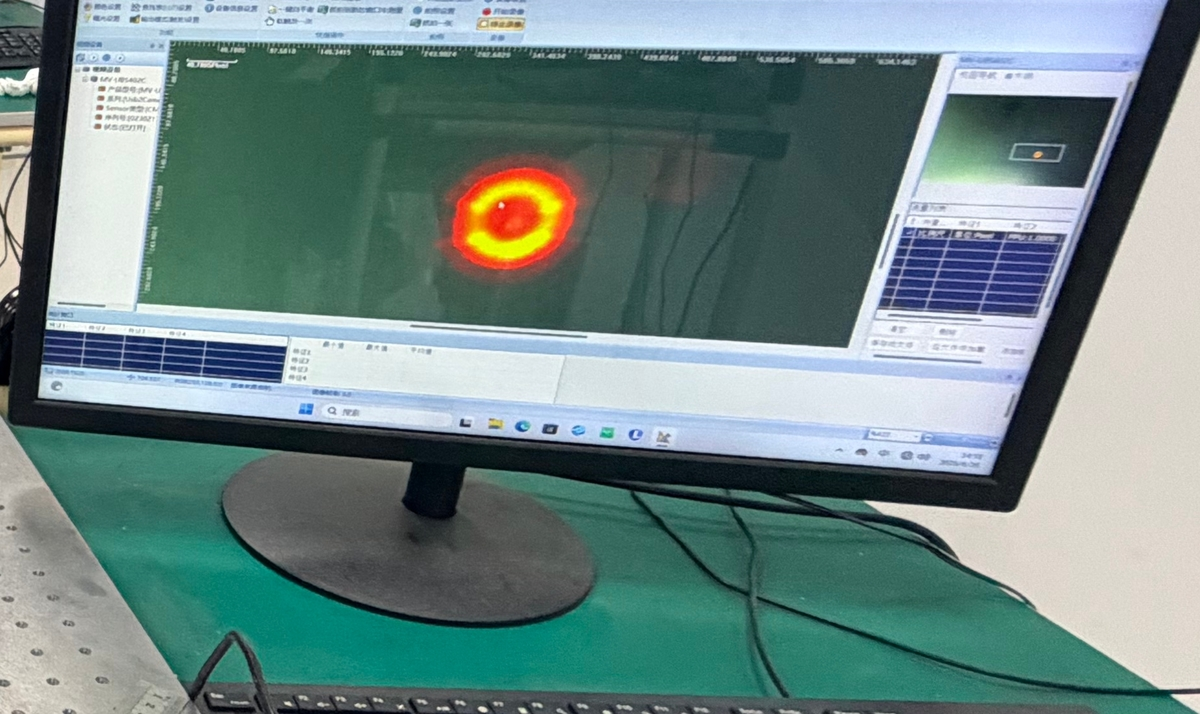
\includegraphics[width=\textwidth]{spherical_ring.jpg}
    \caption{弥散光环}
  \end{subfigure}
  \hfill
  \begin{subfigure}{0.48\textwidth}
    \centering
    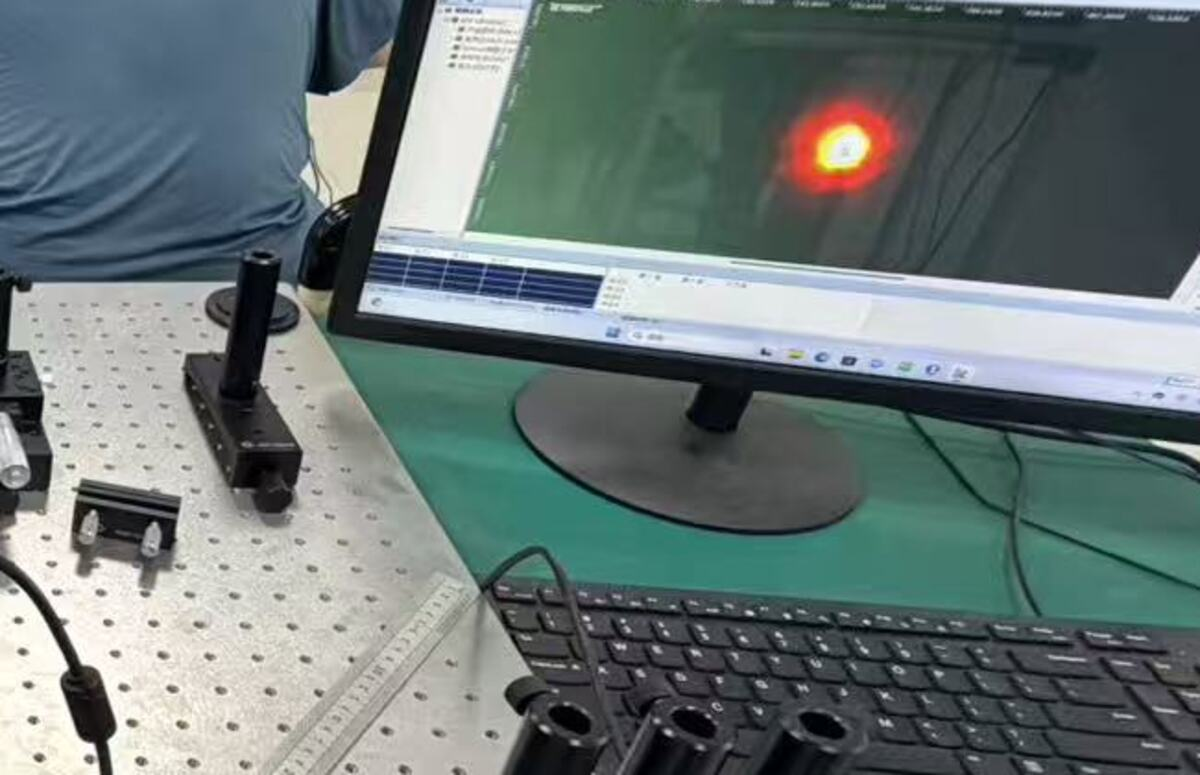
\includegraphics[width=\textwidth]{spherical_focus.jpg}
    \caption{重新调焦后的亮斑}
  \end{subfigure}
  \caption{红光球差测量中的典型星点像}
  \label{fig:spherical}
\end{figure}

\subsection{慧差观察}

在找到焦点后将透镜旋转约 $20^\circ$，CMOS 画面中星点像由近似圆斑变为明显的不对称拖尾。如图\ref{fig:coma}所示，光斑一端亮度集中，另一侧呈扇形扩展，符合慧差的典型形态。

\begin{figure}[H]
  \centering
  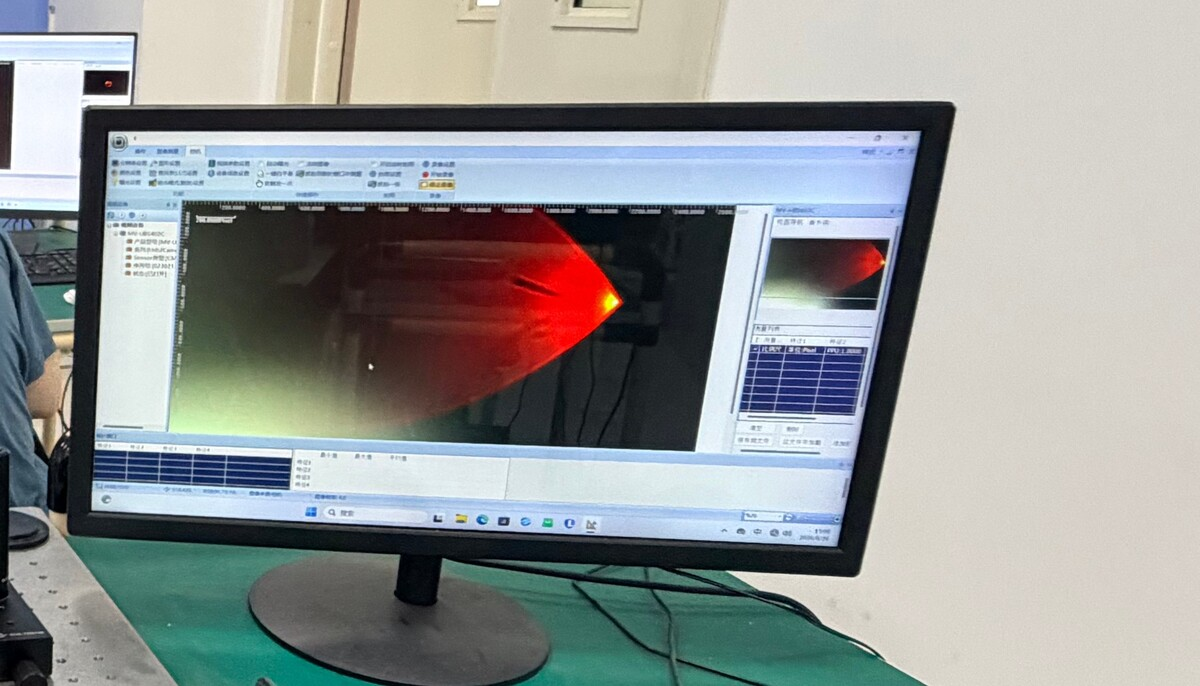
\includegraphics[width=0.82\textwidth]{coma_20deg.jpg}
  \caption{透镜旋转约 $20^\circ$ 时观察到的慧差图样}
  \label{fig:coma}
\end{figure}

\subsection{像散数据处理}

\begin{table}[H]
  \centering
  \caption{像散测量数据}
  \label{tab:astigmatism}
  \begin{adjustbox}{max width=\textwidth}
    \begin{tabular}{ccccc}
      \toprule
      透镜倾角 & 次数 & $X_1$/mm & $X_2$/mm & 像散分离量 $|X_2-X_1|$/mm\\
      \midrule
      $20^\circ$ & 1 & 19.873 & 0.241 & 19.632\\
      $10^\circ$ & 2 & 4.955 & 0.382 & 4.573\\
      $15^\circ$ & 3 & 12.353 & 3.085 & 9.268\\
      \bottomrule
    \end{tabular}
  \end{adjustbox}
\end{table}

由表\ref{tab:astigmatism}可得，不同倾角下像散分离量为
\begin{equation}
  10^\circ:4.573\,\mathrm{mm},\quad
  15^\circ:9.268\,\mathrm{mm},\quad
  20^\circ:19.632\,\mathrm{mm}.
\end{equation}
倾角增大时，两条焦线的轴向分离量明显增大。如图\ref{fig:astigmatism}所示，在透镜倾斜约 $10^\circ$ 时，沿轴向移动相机可分别观察到水平焦线和竖直焦线。

\begin{figure}[H]
  \centering
  \begin{subfigure}{0.48\textwidth}
    \centering
    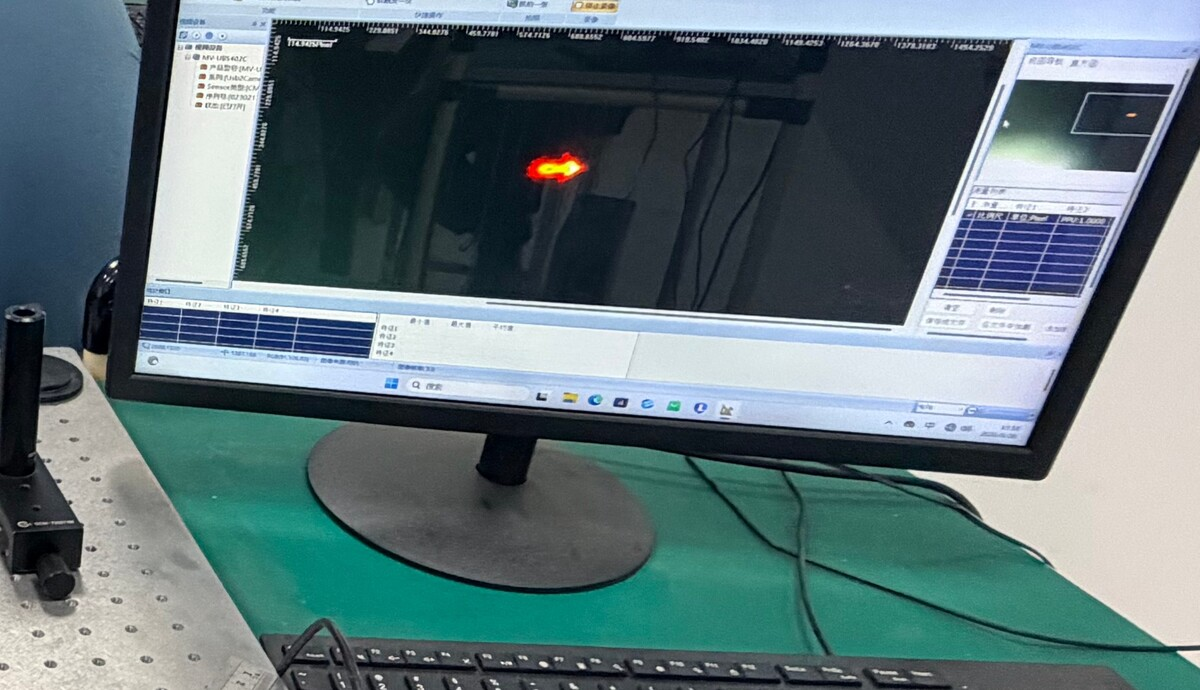
\includegraphics[width=\textwidth]{astig_horizontal.jpg}
    \caption{水平焦线}
  \end{subfigure}
  \hfill
  \begin{subfigure}{0.48\textwidth}
    \centering
    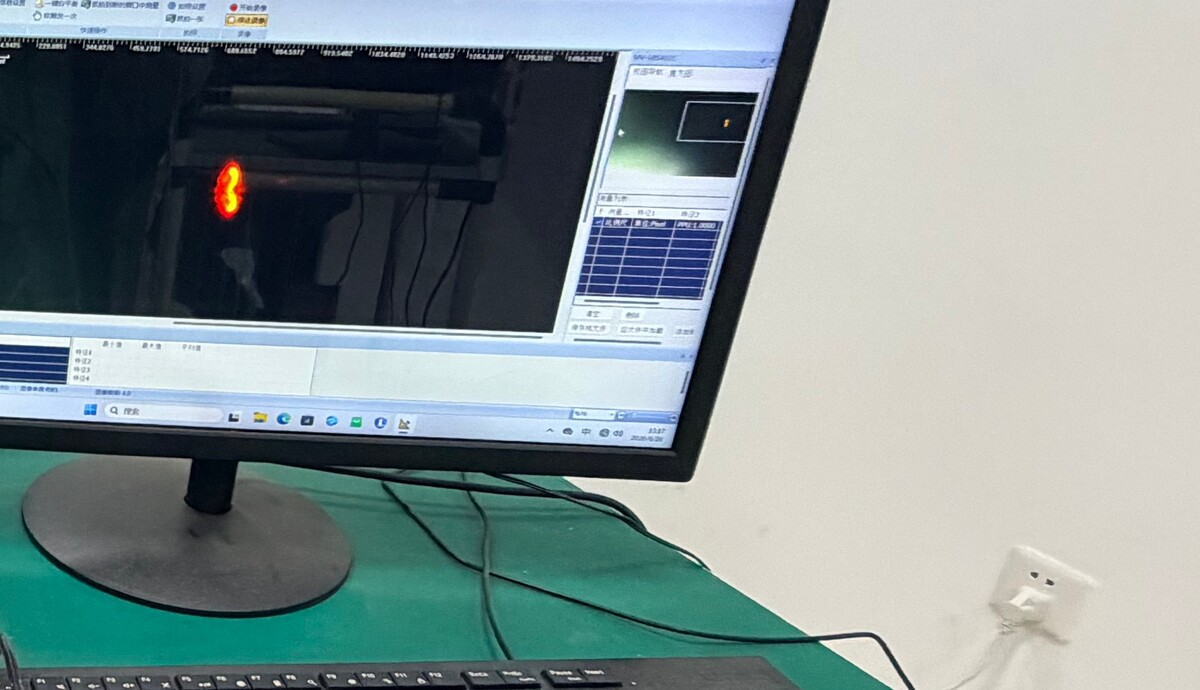
\includegraphics[width=\textwidth]{astig_vertical.jpg}
    \caption{竖直焦线}
  \end{subfigure}
  \caption{透镜倾斜约 $10^\circ$ 时观察到的像散焦线}
  \label{fig:astigmatism}
\end{figure}

\section{实验结果与分析}

位置色差测量表明，红光焦点读数大于蓝光焦点读数，二者平均差为 $3.055\,\mathrm{mm}$。这说明在本实验读数方向上，红光经过透镜后的最佳成像位置比蓝光更远，与红光折射率较小、焦距较长的规律一致。

倍率色差的有符号平均值为 $-19.33\,\mu\mathrm{m}$，其大小约为 $19.33\,\mu\mathrm{m}$。这表示在同一像面处，不同波长光的像点横向位置也存在差异。由于坐标差来自手动点击弥散斑边缘，符号主要反映边缘选取方向，大小更能说明本次实验中倍率色差的量级。

红光球差测量得到轴向分离量 $4.379\,\mathrm{mm}$，垂轴球差 $58.97\,\mu\mathrm{m}$。更换环带光阑后，CMOS 画面从集中亮斑变为弥散光环，再经轴向调焦后重新收缩，说明不同孔径区域的光线焦点不重合，透镜存在明显球差。

慧差观察中，透镜旋转约 $20^\circ$ 后星点像出现不对称拖尾，说明透镜倾斜引入了轴外成像条件。像散测量中，倾角从约 $10^\circ$ 增大到 $20^\circ$ 时，焦线分离量由 $4.573\,\mathrm{mm}$ 增大到 $19.632\,\mathrm{mm}$，说明倾角越大，子午方向和弧矢方向聚焦位置差异越明显。

\section{误差分析}

\begin{enumerate}
  \item \textbf{焦点判定误差。} 星点像在焦点附近并不是突然收缩，而是在一段轴向范围内逐渐变化。若每次对“最小、最亮”的判断不一致，会影响平移台读数。
  \item \textbf{平移台回程误差。} 平移台丝杆可能存在回程间隙。若寻找焦点时移动方向不一致，同一实际位置可能对应略有差别的读数。
  \item \textbf{像素坐标读取误差。} 弥散斑边缘亮度渐变，不存在严格锐利边界；手动点击 $b$、$c$ 坐标时，边缘选取标准不同会直接影响倍率色差和垂轴球差。
  \item \textbf{光路共轴误差。} 光源、平行光管、光阑、透镜和 CMOS 相机若没有严格共轴，光斑会发生偏移或倾斜，测得的像差中会混入装调误差。
  \item \textbf{换光源和换光阑的扰动。} 色差测量需要更换蓝光、红光 LED，球差测量需要更换环带光阑。若更换过程中元件中心位置或高度发生改变，会影响焦点读数和光斑形状。
  \item \textbf{倾角估计误差。} 慧差和像散观察中透镜倾角主要由机械刻度和人工调节确定，实际角度可能与记录值有偏差，因此像散随倾角变化更适合做趋势分析。
\end{enumerate}

\section{实验结论}

本实验用星点法测量并观察了透镜的典型像差。色差测量中，蓝光焦点平均读数为 $11.438\,\mathrm{mm}$，红光焦点平均读数为 $14.492\,\mathrm{mm}$，位置色差平均值为 $3.055\,\mathrm{mm}$。倍率色差的大小约为 $19.33\,\mu\mathrm{m}$，说明不同波长光既有轴向焦点差异，也有横向像高差异。

红光球差测量中，不同环带光阑对应焦点的轴向分离量为 $4.379\,\mathrm{mm}$，垂轴球差为 $58.97\,\mu\mathrm{m}$。实验中观察到弥散光环和重新调焦后的亮斑，说明不同孔径区域的光线会聚位置不一致。

在透镜倾斜条件下，实验观察到明显慧差拖尾和像散焦线。像散分离量随倾角增大而明显增大，约 $10^\circ$、$15^\circ$、$20^\circ$ 时分别为 $4.573\,\mathrm{mm}$、$9.268\,\mathrm{mm}$ 和 $19.632\,\mathrm{mm}$。这表明星点法能够通过光斑形状和轴向位置变化直观反映透镜色差、球差、慧差和像散。

\appendix
\renewcommand{\thefigure}{\Alph{section}-\arabic{figure}}
\renewcommand{\thetable}{\Alph{section}-\arabic{table}}
\section{原始数据记录}

原始数据记录页中含手写测量数据，正文已将其整理为三线表。按实验报告写作规范，原始记录页在附录中保留，如图\ref{fig:raw-data-01}和图\ref{fig:raw-data-02}所示。

\begin{figure}[H]
  \centering
  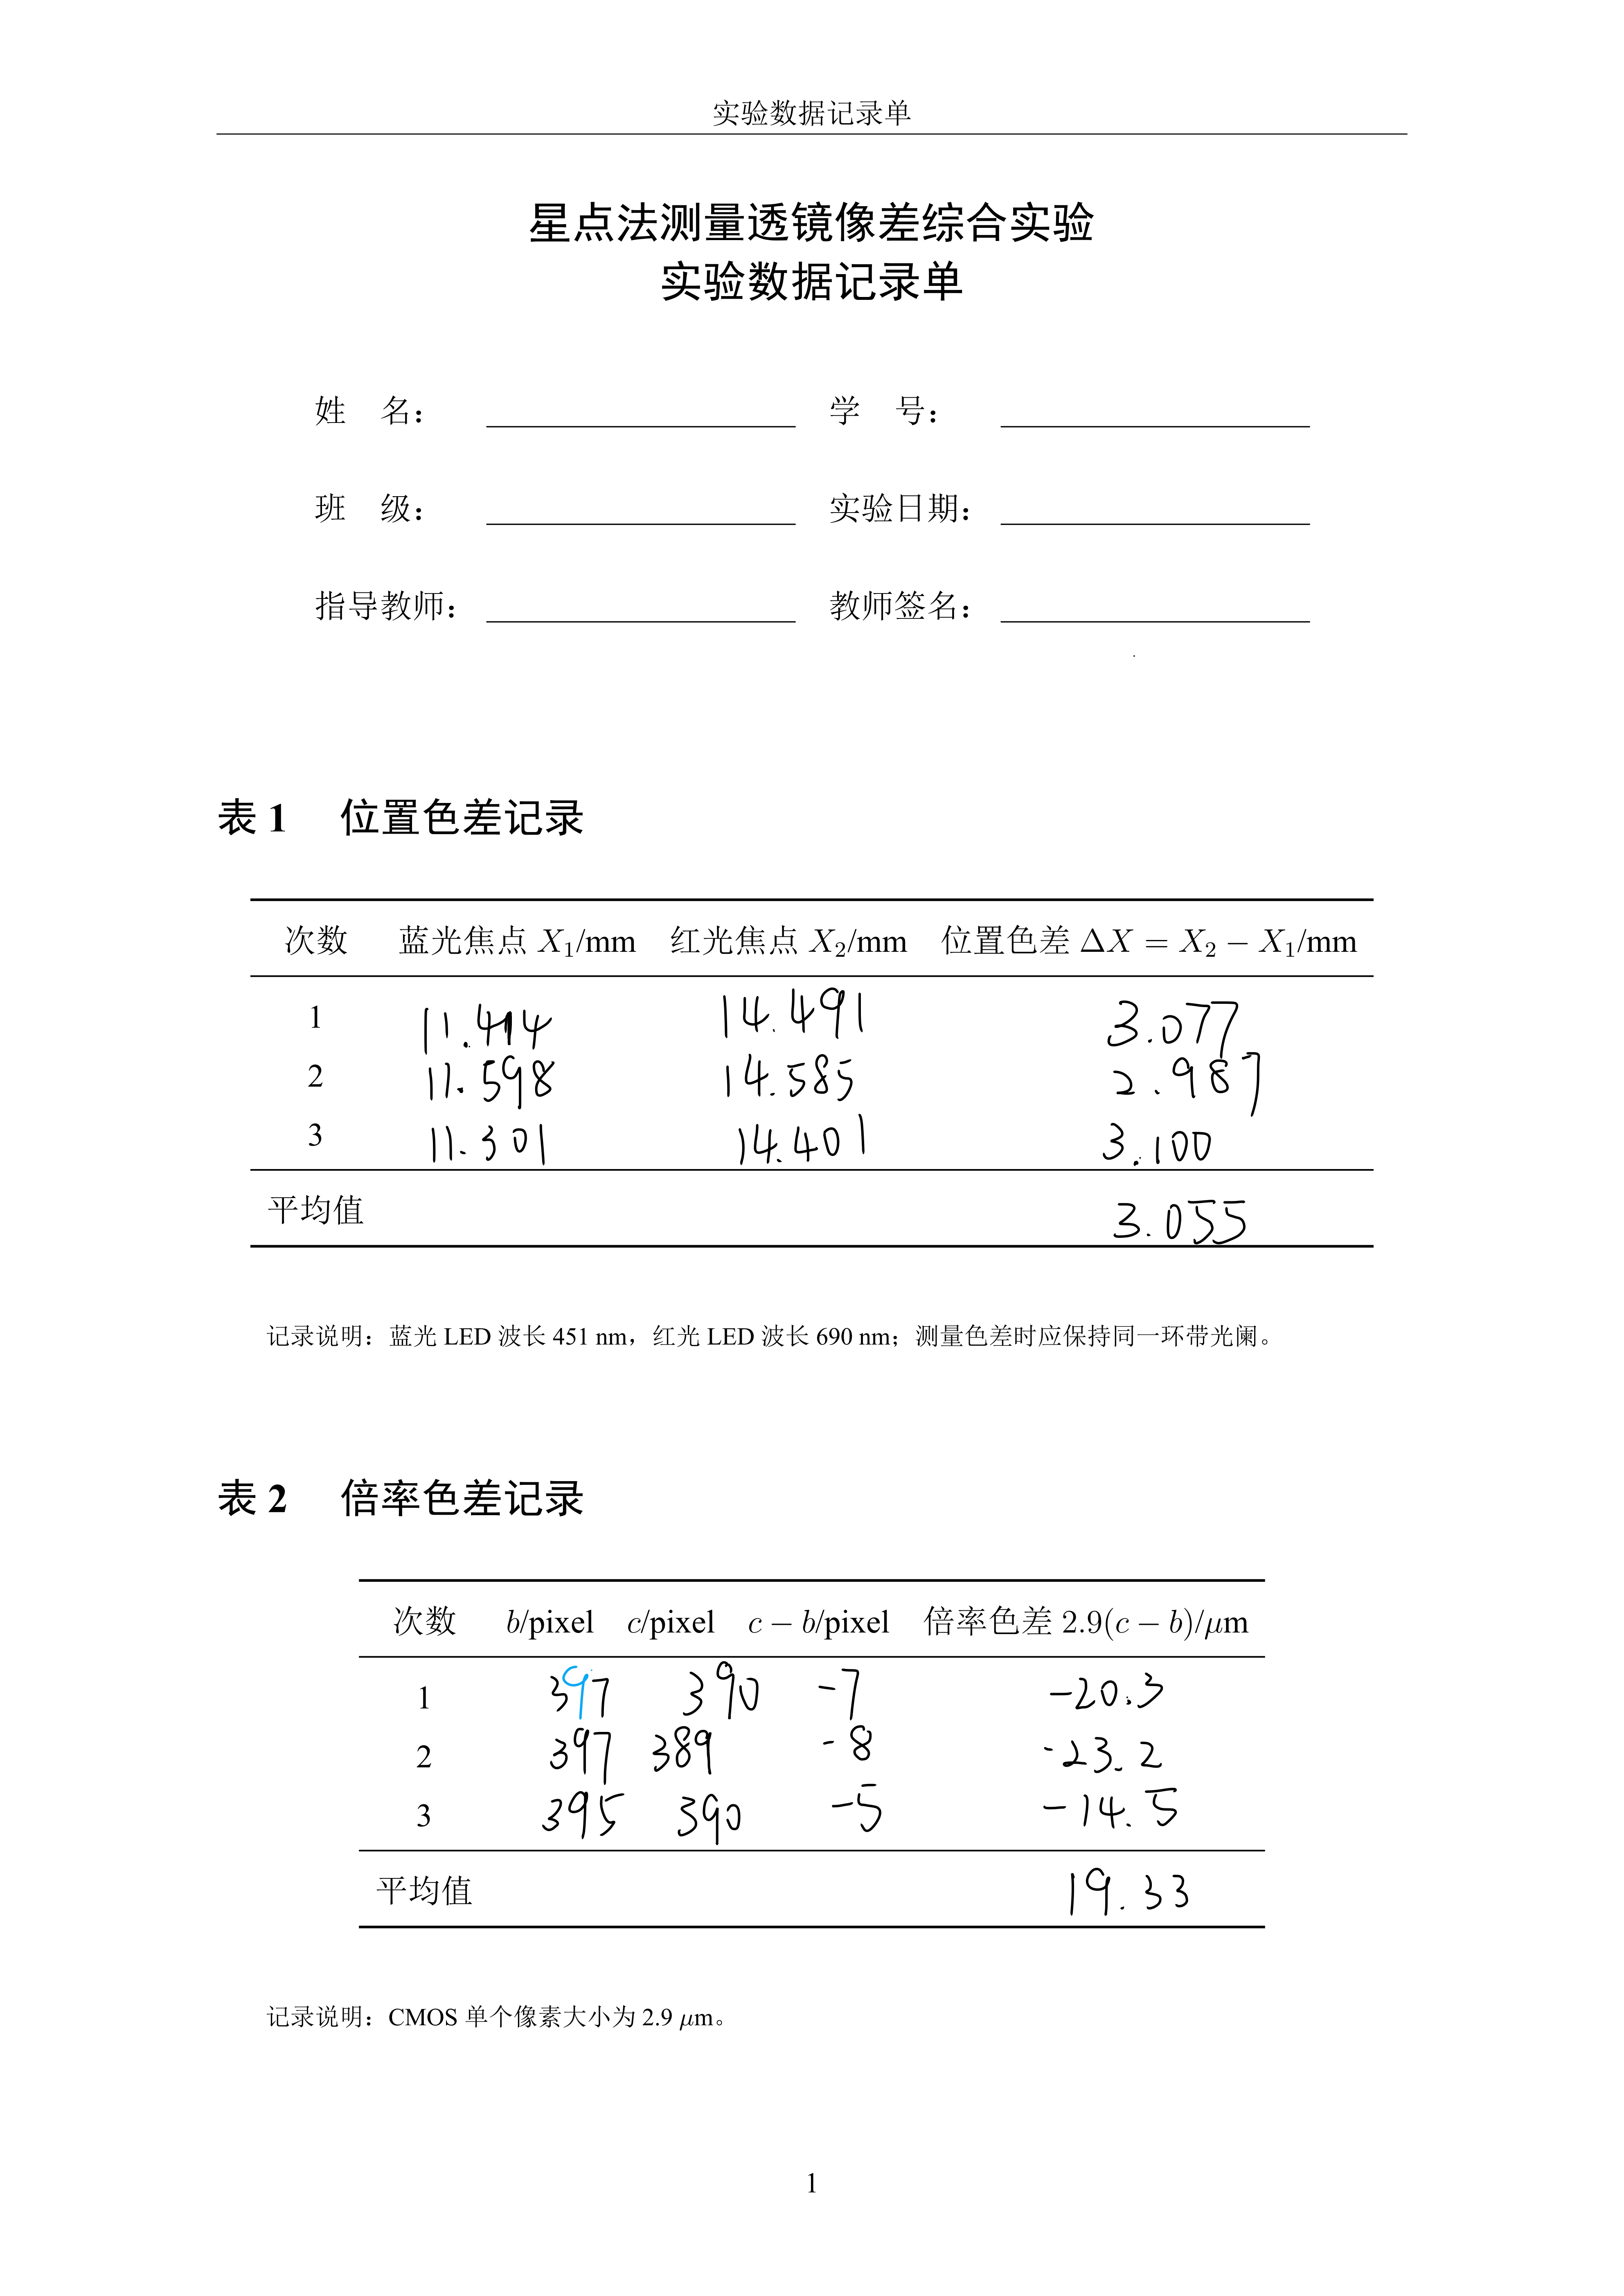
\includegraphics[width=0.82\textwidth]{raw_data_01.png}
  \caption{原始数据记录第 1 页}
  \label{fig:raw-data-01}
\end{figure}

\begin{figure}[H]
  \centering
  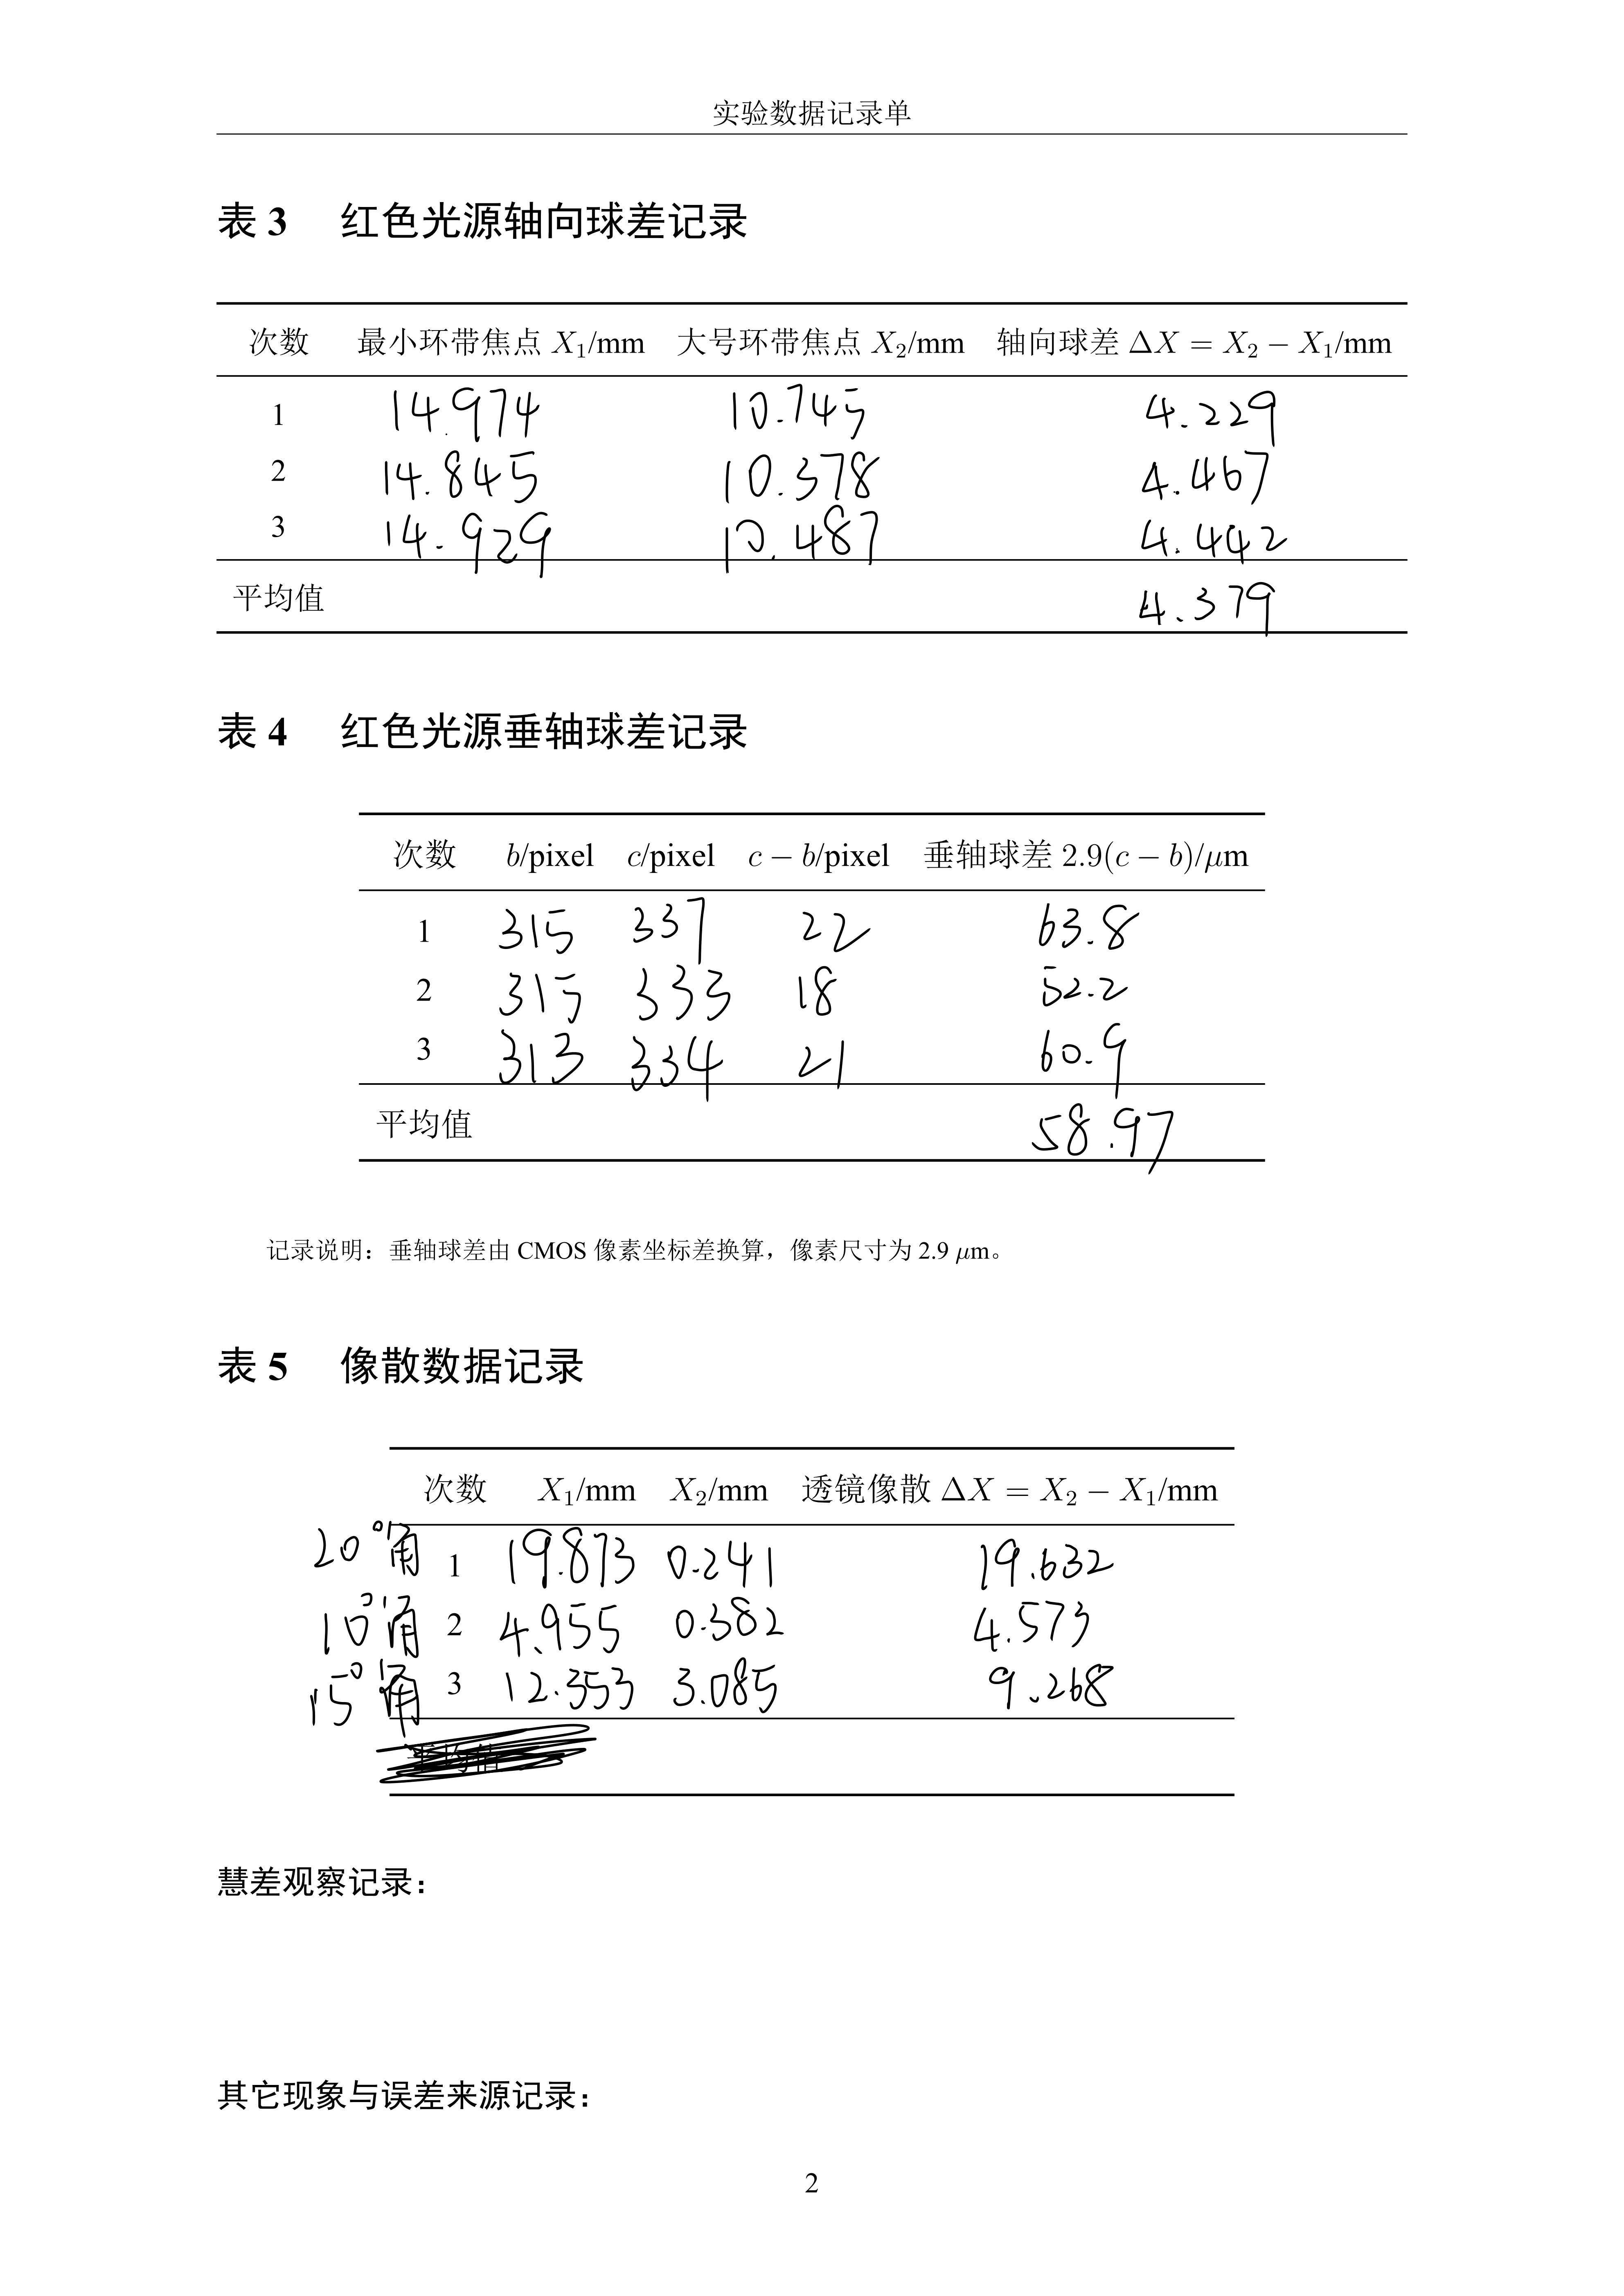
\includegraphics[width=0.82\textwidth]{raw_data_02.png}
  \caption{原始数据记录第 2 页}
  \label{fig:raw-data-02}
\end{figure}

\end{document}

在某一焦面上，大号环带光阑产生的弥散环还可用于估计垂轴球差。若弥散环边缘与参考像素坐标差为 $c-b$，则垂轴球差为
\begin{equation}
  \Delta h=2.9(c-b)\,\mu\mathrm{m}.
\end{equation}

\subsection{慧差与像散}

慧差（coma）常由轴外光束或透镜倾斜引起。透镜倾斜后，不同孔径区域光线在像面上的放大率和会聚位置不同，星点像不再圆对称，而呈现一端明亮、一端拖尾的彗星状图样。

像散（astigmatism）是子午面和弧矢面内光线分别在不同轴向位置聚焦造成的像差。沿光轴移动 CMOS 相机时，会先后观察到两个近似互相垂直的线状焦斑。两条焦线对应平移台读数的差值大小反映像散程度：
\begin{equation}
  |\Delta X|=|X_2-X_1|.
\end{equation}
